\documentclass[12pt]{article}
%\documentclass[article,12pt]{amsart}


%%%%%%%%%%%%%%%%%%%%%%%%%%%%%%%%%%%%%%%%%%%%
% The % is the comment character.
% If you use emacs as a text editor, then the command
% M-x global-font-lock-mode 
% will turn on command highlighting
%%%%%%%%%%%%%%%%%%%%%%%%%%%%%%%%%%%%%%%%%%%%

%%%%%%%%%%%%%%%%%%%%%%%%%%%%%%%%%%%%%%%%%%%
% Here are packages for fonts, symbols, and graphics

%\usepackage{mathrsfs}
\usepackage{amssymb}
\usepackage[english]{babel}
\usepackage{graphicx}
\usepackage{versions}
\usepackage{amsmath}
\usepackage{appendix}

\usepackage{color} %
\usepackage{times} %
\usepackage{amsthm} %
\usepackage{amsfonts} %
\usepackage[small]{caption} %
\usepackage{natbib} %
\usepackage[letterpaper]{geometry} %
%\usepackage{hyperref} %


\usepackage{colortbl}
\definecolor{myGrey}{rgb}{.7,.75,.75}

\bibpunct{(}{)}{;}{a}{}{,} %
\setlength{\leftmargini}{4.8mm} %
\setlength{\leftmargini}{4.8mm} %
\setlength{\leftmarginii}{4.8mm} %
\geometry{hmargin={1.34in,1.14in}, vmargin={1.02in,.99in}}



%%%%%%%%%%%%%%%%%%%%%%%%%%%%%%%%%%%%%%%%%%%
% Here are useful environments. Use them by typing, e.g.
%  \begin{thm} Statement of theorem \end{thm}
% Often followed at some point by \begin{proof} Proof \end{proof}

% \newtheorem{thm}{Theorem}[section]
% \newtheorem{lem}[thm]{\textbf Lemma}
% \newtheorem{cor}[thm]{Corollary}
% \newtheorem{prop}[thm]{\textbf Proposition}
% \newtheorem{crit}[thm]{Criterium}
% \newtheorem{alg}[thm]{Algorithm}


%%%%%%%%%%%%%%%%%%%%%%%%%%%%%%%%%%%%%%%%%
% Here is a different environment. Use it the same way and see what it looks
% like

%\theoremstyle{definition}

% \newtheorem{defn}[thm]{Definition}
% \newtheorem{conj}[thm]{Conjecture}
% \newtheorem{exmp}[thm]{\textbf{Examples}}
% \newtheorem{exe}[thm]{\textbf{Example}}
% \newtheorem{prob}[thm]{Problem}

%%%%%%%%%%%%%%%%%%%%%%%%%%%%%%%%%%%%%%%%%
% Here is a different environment. Use it the same way and see what it looks
% like

% \theoremstyle{remark}

% \newtheorem{rem}[thm]{\textbf{Remark}}
% \newtheorem{note}[thm]{Note}
% \newtheorem{claim}[thm]{Claim}  \renewcommand{\theclaim}{}
% \newtheorem{summ}{Summary}      \renewcommand{\thesumm}{}
% \newtheorem{case}{Case}
% \newtheorem{ack}{ACKNOWLEDGEMENTS}        \renewcommand{\theack}{}

%%%%%%%%%%%%%%%%%%%%%%%%%%%%%%%%%%%%%%%
% Some macros for frequently used commands

\def\R{\mathbb{R}}
\def\to{\rightarrow}
\def\der#1#2{\frac{\partial #1}{\partial #2}}  %% This is a partial derivative
\def\ip#1#2{\left<#1,#2\right>}  %% This is an inner product
\def\inv#1{\frac{1}{#1}}


%%%%%%%%%%%%%%%%%%%%%%%%%%%%%%%%%%%%%%%
% Formatting stuff

\renewcommand{\baselinestretch}{1.5}
\setlength{\textwidth}{167mm} \addtolength{\hoffset}{-22mm}

%%%%%%%%%%%%%%%%%%%%%%%%%%%%%%%%%%%%%%
% No box at the end of proofs

%\renewcommand{\qedsymbol}{}

%%%%%%%%%%%%%%%%%%%%%%%%%%%%%%%%%%%%%%
% Now for the actual document

%%%
%%%%%%%%%%%%%%macros for this particular document
%%%

\def\Z{\mathbb{Z}}


%I am so confused.  \alpha_1, \sigma_1, \phi_1 are broken but _2 work. what?
\def\la{\lambda}
\def\ka{\kappa}
\def\elrt#1#2{ e^{- \la (#1 -#2)rt} }

%\includeversion{self}
\excludeversion{self}

% DO NOT DELETE the following line.  It is used by R package documentation.
% \VignetteIndexEntry{ MCMC on Restricted Immigration Model }
% DO NOT DELETE the above line
\title{DOBAD Package: 
  Gibbs Sampling MCMC of Linear Birth-Death Chain with Partial Data}

\author{Charles Doss}
\date{September 2009}

\usepackage{Sweave}
\begin{document}



\begin{titlepage}
\maketitle
\end{titlepage}


\vspace{-3.7mm} %






\part{Estimating Rates for Linear Birth-Death chain via Gibbs Sampler MCMC by
  Exact Conditional Simulation}

We are demonstrating the use of the
\begin{verb}
DOBAD
\end{verb}
package's capability to do Bayesian estimation of the rate parameters
for a linear Birth-Death chain, given partial observations, using 
the methods of \citet{DSHKM2010EM}.  Call the
chain $\{X(t)\}_{t \in \R}$, and its birth rate $la$ and its death
rate $\mu$.  We fix $\beta \in \R$ and constrain $\nu$, the
immigration rate, to be $\nu=\beta la$.  We will denote $\theta = (la,
\mu)$.  The data is the value of the process at a finite number of
discrete time points.  That is, for some fixed times $0=t_0, t_1,
\ldots, t_n$, we see the state of the process, $X(t_i)$.  Thus the
data, $D$, is $2$ parts: a vector of the times $t_i$, $i= 0, \ldots,
n$ and a vector of states at each of those times, $s_i$, for $i=0,
\ldots, n$ (where $X(t_i) = s_i$.  The gamma prior is the conjugate
prior if we observed the chain continuously instead of partially.  The
way we proceed, then, is to use independent Gamma priors on the
$\lambda$ and $\mu$ and augment the state space for our MCMC to include
the entire chain $\{X_t\}_{t \in [0,t_n]}$ by conditionally 
sampling $\{X_t\}_{t \in [0,t_n]};\theta | D$.

First we generate the underlying process and the ``data'', set our
prior parameters, and compute some summary statistics of the fully
observed and partially observed processes.
\begin{Schunk}
\begin{Sinput}
> library(DOBAD)
> initstate = 7
> set.seed(112)
> T = 5
> L <- 0.2
> mu <- 0.4
> beta.immig <- 0.987
> trueParams <- c(L, mu, beta.immig)
> names(trueParams) <- c("lambda", "mu", "beta")
> dr <- 1e-10
> n.fft <- 1024
> delta <- 1
> dat <- birth.death.simulant(t = T, lambda = L, mu = mu, nu = L * 
+    beta.immig, X0 = initstate)
> fullSummary <- BDsummaryStats(dat)
> fullSummary
\end{Sinput}
\begin{Soutput}
   Nplus   Nminus Holdtime 
12.00000 14.00000 26.73947 
\end{Soutput}
\begin{Sinput}
> MLEs <- M.step.SC(EMsuffStats = fullSummary, T = T, beta.immig = beta.immig)
> MLEs
\end{Sinput}
\begin{Soutput}
lambdahat     muhat 
0.3788540 0.5235706 
\end{Soutput}
\begin{Sinput}
> partialData <- getPartialData(seq(0, T, delta), dat)
> observedSummary <- BDsummaryStats.PO(partialData)
> observedSummary
\end{Sinput}
\begin{Soutput}
   Nplus   Nminus Holdtime 
       3        5       28 
\end{Soutput}
\begin{Sinput}
> L.mean <- 1
> M.mean <- 1.1
> aL <- 0.02
> bL <- aL/L.mean
> aM <- 0.022
> bM <- aM/M.mean
> print(paste("Variances are", aL/bL^2, "and", aM/bM^2))
\end{Sinput}
\begin{Soutput}
[1] "Variances are 50 and 55"
\end{Soutput}
\begin{Sinput}
> N = 100
> burn = 0
\end{Sinput}
\end{Schunk}

Now we run the MCMC.  It is set to run only $100$ iterations, which is
obviously not enough for estimation, but does demonstrate the code.

\begin{Schunk}
\begin{Sinput}
> timer <- system.time(theMCMC <- BD.MCMC.SC(Lguess = L.mean, Mguess = M.mean, 
+    alpha.L = aL, beta.L = bL, alpha.M = aM, beta.M = bM, beta.immig = beta.immig, 
+    data = partialData, burnIn = burn, N = N))
\end{Sinput}
\begin{Soutput}
[1] "BD.MCMC.SC: On the  30 th iteration params are  0.50525582705533 0.643698845152378"
[1] "BD.MCMC.SC: On the  60 th iteration params are  0.408368213696412 0.406325363782436"
[1] "BD.MCMC.SC: On the  90 th iteration params are  0.271395764173334 0.513698779398225"
\end{Soutput}
\begin{Sinput}
> mean(theMCMC[, 1])
\end{Sinput}
\begin{Soutput}
[1] 0.4252525
\end{Soutput}
\begin{Sinput}
> mean(theMCMC[, 2])
\end{Sinput}
\begin{Soutput}
[1] 0.5536474
\end{Soutput}
\begin{Sinput}
> L
\end{Sinput}
\begin{Soutput}
[1] 0.2
\end{Soutput}
\begin{Sinput}
> mu
\end{Sinput}
\begin{Soutput}
[1] 0.4
\end{Soutput}
\begin{Sinput}
> timer
\end{Sinput}
\begin{Soutput}
   user  system elapsed 
 11.253   0.060  13.002 
\end{Soutput}
\begin{Sinput}
> options(continue = " ")
\end{Sinput}
\end{Schunk}

\begin{Schunk}
\begin{Sinput}
> hist(theMCMC[, 1], freq = FALSE, breaks = 20, xlab = "Lambda", 
     ylab = "Density", main = "Posterior of Lambda")
> Lmean <- mean(theMCMC[, 1])
> abline(col = "red", v = Lmean)
> abline(col = "purple", v = L.mean)
> x <- seq(from = 0, to = 1, by = 0.01)
> y <- dgamma(x, shape = aL, rate = bL)
> lines(x, y, col = "blue")
\end{Sinput}
\end{Schunk}
\begin{figure}
  \begin{center}
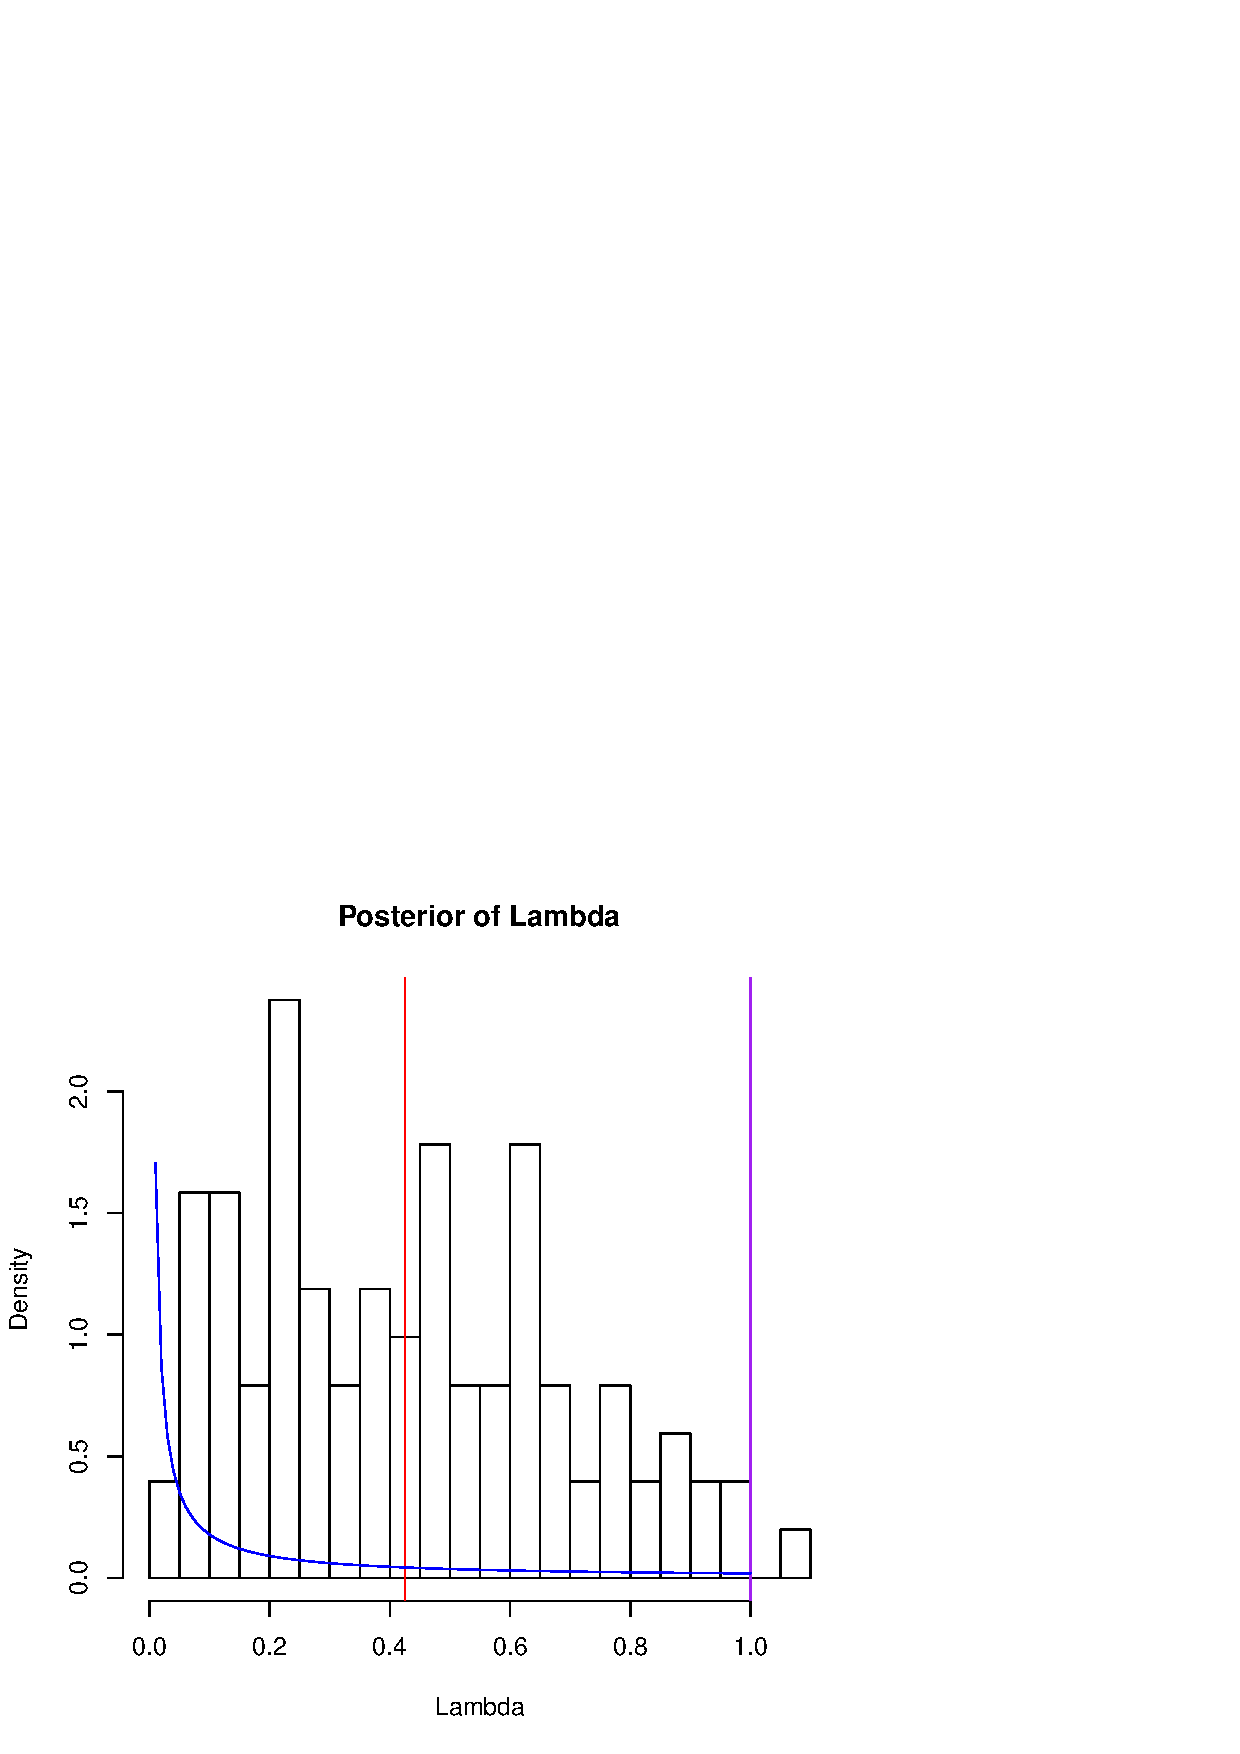
\includegraphics{BD_MCMC-lambdaPlot}
\end{center}
\caption{Posterior Density Estimation of Lambda}
\label{fig:lambdaPosterior}
\end{figure}

\begin{Schunk}
\begin{Sinput}
> hist(theMCMC[, 2], freq = FALSE, breaks = 20, xlab = "Mu", ylab = "Density", 
     main = "Posterior of Mu")
> Mmean <- mean(theMCMC[, 2])
> abline(col = "red", v = Mmean)
> abline(col = "purple", v = M.mean)
> x <- seq(from = 0, to = 1, by = 0.01)
> y <- dgamma(x, shape = aM, rate = bM)
> lines(x, y, col = "blue")
\end{Sinput}
\end{Schunk}
\begin{figure}
  \begin{center}
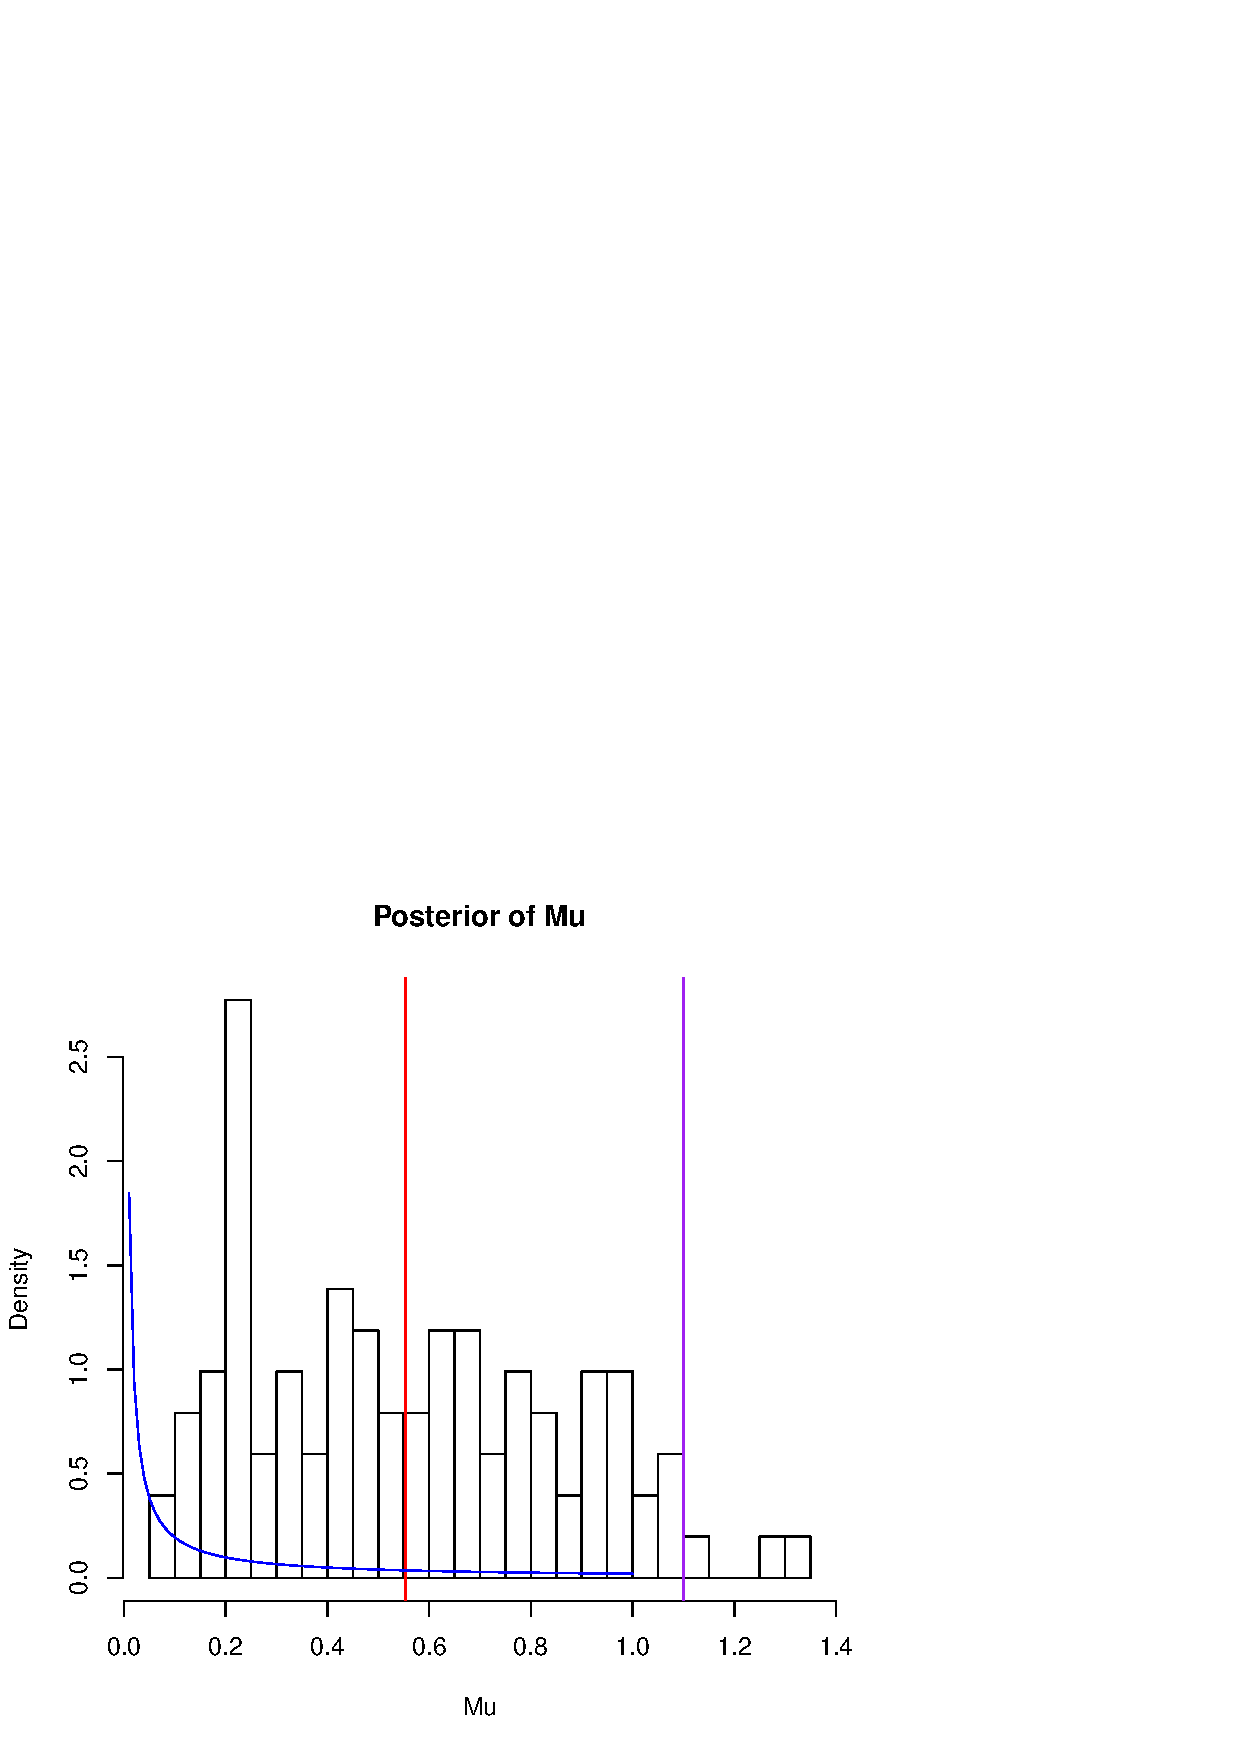
\includegraphics{BD_MCMC-muPlot}
\end{center}
\caption{Posterior Density Estimation of Mu}
\label{fig:muPosterior}
\end{figure}



\bibliographystyle{biom} %
\bibliography{DOBADbiblio}


\end{document}







